\paragraph{}During recent years, we have witnessed an explosion on the Internet of Thing (IoT) in term of the number and types of physical devices. However, there are many limitations of these devices regarding their computing power, storage, and connection. They affect on-device processing of sensed data significantly. Centralized treatment of IoT data has proven challenging for many use cases demanding real time response. This paper aims at augmenting sensor data processing using the concept of virtual sensors. We propose a scalable virtual sensor framework that supports building a logical data-flow (LDF) by visualizing either physical sensors or custom virtual sensors. The process produces high-level information from the sensed data that can be easily perceived by machines and humans. A web-based virtual sensor editor (VSE) is also implemented on the top of the framework to simplify creation and configuration of the LDF. The VSE supports cross-platform and real-time verification for composed LDF. The paper also presents a catalog of supported virtual sensor type along with preliminary performance study.

\section{Introduction}
The Internet of Things (IoT) is expected to bring connectivity to every object in the physical world. From connected cars, buildings and cities, the IoT creates many opportunities in various domains~\cite{AlFuqahaGuizaniMohammadiAledhariAyyash2015}. According to Wikibon report~\cite{Floyer2013}, by the end of 2020, 212 billion IoT smart objects are expected to be deployed worldwide. Despite the rapid growth, the IoT is still facing some major challenges relating interoperation, performance, data reliability. On the contrary, the cloud computing environment offers a massive ability in term of computing and storage. Thus, integrating the IoT with Cloud technology is expected to provide scalable storage and sensing services enabling unlimited IoT device connecting to the Internet, which is called the CloudIoT paradigm~\cite{BottaDonatoPersicoPescape2014}.\\

However, there are critical challenges to archive higher-level information from raw data of the physical device. Even the exponential growth of IoT smart objects in term of power and functionality, certain situations cannot be handled at the device level. For instance: (i) a comprehensive query for checking the average of humidity in a region. This query may request all data of humidity sensor deployed in the corresponding area. (ii) Predicting missing data based on the historical data. To handle these situations, virtualization of the physical sensor in cloud environment, namely Virtual Sensor (VS), is considered as a practical approach. VS is a logical reflection of one or a set of physical sensors on the Cloud platform and is able to handle complex tasks which cannot be performed on physical sensors~\cite{Julien2006}~\cite{Crowcroft2012}. The key aspect of VS is to facilitate and enrich the functionalities of physical sensors at the software level to adapt to different purposes and scenarios~\cite{GuptaMukherjee2016}. \\

In this paper, we present a scalable virtual sensor framework (sVSF). It simplifies creating and configuring VSs with the programmable operators (rule, formula or function). These VSs are linked together to be a logical data-flow that enables to produce the high-level information over collected data. On the top of the framework, a Virtual Sensor Editor (VSE) is also implemented to facilitate building and configuring the LDF by offering the drag-drop actions on HTML5 web interface. In order to archive scalability and performance, sVSF is implemented based on clustering architecture along with various strategies such as executing LDF following asynchronous model, using No-SQL database to store and query data. \\

Our framework supports various types of virtual sensors at Infrastructures as a Service (IaaS) and Platform as a Service (PaaS) such as singular, accumulator, aggregator, selector, qualifier, context-qualifier, and simple predictor~\cite{SBoseAGuptaSAdhikaryN2015}. In the sVSF, VSs are treated as physical sensors. The output data of VS is stored in the database in the same way as physical. Thus, each VS carries the historical data which is valuable for further data analyzing. Furthermore, the proposed framework remarkably fits for Low Power Wide Area Networking (LPWAN) scenario where band width (12 bytes in SIGFOX and up to 250 bytes in LORA), and data rate (typically 10 kilobits per seconds) are limited~\cite{AdelantadoVilajosanaTusetMartinezMeliaSegui2017}. These restrictions reduce the quantity of collected data that affects directly on further data analysis and context-awareness in term of accuracy and trustworthiness. \\

On the top of the framework, sVSF offers a cross-platform development environment for the virtual sensor by enabling HTML5 technology. The lower layers take principal responsibility to process and generate high-level information based on composed LDF. In order to enhance scalability and performance, the core framework is implemented following clustering architecture using Nodejs language. Our paper has four highlighted contributions:
\begin{itemize}
    \item Identifying the limitations of current virtual sensor framework in term of VS functionality and usability.
    \item Reviewing the concept of virtual sensor and its taxonomy.
    \item Presenting a scalable virtual sensor framework to increase information quality from sensed data, and implementing clustering model along with various strategies to archive high scalability and performance. 
    \item A cross-platform development tool for virtual sensor, namely virtual sensor editor, is also offered to speed up designing logical data-flow.
\end{itemize}


\section{Background analysis}

In this section, we review virtual sensor and current virtual sensor framework in the IoT. Their limitations are also identified. At the end of the section, we present our motivations to bridge the gaps by delivering a scalable IoT virtual sensor framework.\\

As a definition in~\cite{GuptaMukherjee2016}, a virtual sensor reflects a physical sensor that is able to obtain and represent data on cloud. Following~\cite{MadriaKumarDalvi2014}, a virtual sensor is an emulation of a physical sensor which collects its data from underlying physical sensors. There are many ways to define and categorize virtual sensor, in~\cite{GuptaMukherjee2016}, the authors also separate virtual sensor into two types: (i) Task level: represents the physical sensor as a virtual object that could be processed, calculated. (ii) Node level: represents a subset of physical sensor as a virtual topology.  In~\cite{MadriaKumarDalvi2014}, virtual sensor is classified into four typical types: (i) One-to-Many: One physical sensor is represented by many virtual sensors. (ii) Many-to-One: One and more physical sensor is presented by one virtual sensor. (iii) Many-to-Many: This is the combination of two under types. (iv) Derived: One virtual sensor can represent different physical sensor types. While in other types, the virtual sensor only represents the same physical device type. At the IaaS level,~\cite{BoseGuptaAdhikaryMukherjee2015} categorizes virtual sensor based on their offering services. Therefore, in the IoT, the definition and taxonomy of the virtual sensor are chaos and heterogeneous. \\

The authors of~\cite{al2013} propose a web-based virtual sensor editor tool to facilitate designing virtual sensor process. This tool visually aggregates either the physical sensors or customized virtual sensors. It also supports calculating and visualizing real-time sensor values on graphic charts. VSs are created by aggregating physical sensors. The graphic interface supports native HTML5 drag-drop and real-time virtual sensor evaluation. As a result of HTM5 characteristics and call-by-need strategy, this tool enables cross-platform and scalability. Similarly, the authors of~\cite{JeongJooHongShinLee2015} present a web-based interactive framework to visualize and authorize sensors as well as actuators for indoor scenario. Each IoT Thing serves as a node, which is visualized within a 3D indoor scene. Thus, the end-user can monitor, link and program sensors and actuators respectively. This framework works based on event handling model which treats incoming data as an event. In order to handle complex events, that must be processed on multiple sensors; the author proposes a hierarchical graph for visual summarizing sensors, actuators and their relations. \\

In the IoT environment, physical sensors are distributed and affected by many adverse factors. Thus, sensed data need to be processed, filtered and transformed for precise measurement and providing high-level information. Many middleware platforms are designed to process the IoT data on either multi-sensors or multi-stream~\cite{Julien2014}~\cite{LHuFWangJZhouK2015}. These works aim to improve the information quality of data coming from heterogeneous data sources. In the same scope, the authors of~\cite{BrunelliGalloBenini2016} present a virtual sensor environment that can handle real-time sensing data processing. This approach uses Complex Event Processing (CEP) as a virtual sensor engine. Their main contributions are to take the benefit from CEP and allow the user to define the custom analytic algorithm along with data analysis block on the incoming data. The authors of~\cite{GuptaMukherjee2016} address solving major challenges about implementing virtual sensor at Software as a service (SaaS) and Platform as a service (PaaS) level. They propose explicit sensor-cloud architecture with four separate modules to handle specific tasks such as sensing, processing, storing and communicating. Each module is equipped an API supporting the end-user building applications and sharing sensed data to either the IoT users or services.\\

The limitations of state-of-the-art are given below.
\begin{itemize}
    \item In~\cite{al2013}, we notice limited functionalities for the virtual sensor. These functions are only able to perform on incoming data. There is no discussion regarding virtual sensor types and which types are supported by their tool.
    \item The authors of~\cite{JeongJooHongShinLee2015} have not shown how to configure the algorithm of CEP. They also do not offer a graphic interface to facilitate the configuration process of data analysis block for end-user. Likewise, the works of~\cite{Julien2014}~\cite{LHuFWangJZhouK2015} more focus on services and implementation than simplifying configuration process at the user level.
    \item The work of~\cite{BrunelliGalloBenini2016} just focuses on the indoor scenario. There is no mention on the mechanism to create and configure a custom virtual sensor as well as an actuator.
\end{itemize}
From all points above, there is not a comprehensive virtual sensor framework proposing an effective web-based interface along with a robust backend. Utilization of virtual sensor to present historical data is also not mentioned. Our framework is designed and implemented to mitigate their limitations.

\section{Contribution}
\paragraph{}In this section, we present the definition and taxonomy of the virtual sensor as well as our virtual sensor framework architecture, which is designed as a modularized layered application. Such framework operates over clustering architecture and asynchronous model to maximize scalability and performance. At the end of the section, we describe the work-flow of the proposed framework in specific deployment scenarios to emphasize its benefit.
\subsection{Virtual Sensor}
We define the virtual sensor as a virtual object. Such object is equipped an operator to perform specific functionalites. In our framework, we support three type of operator including rule, formula and function. We also proposed a new taxonomy of the virtual sensor based on its operator. For instance, a virtual sensor is labelled an “Accumulator” type if its operator contains accumulated functions. The following is the list of supported virtual sensor type:
\begin{itemize}
    \item \textbf{\textit{Singular}}: This type allows to perform a one-to-one mapping between the physical sensor and its reflected interface in cloud side. Through this virtual interface, the end-user can configure sensor configuration to obtain the data from a physical sensor. At the first stage, the sensor configuration is stored as a sensor driver that is selected by the user via VSE.
    \item \textbf{\textit{Accumulator}}: A virtual sensor could perform accumulated function on its sensing data within a particular duration. For example, a rainfall physical sensor uses the counter value to identify the rainwater volume. An accumulator VS is useful to present rainwater volume within 24 hours by accumulating on this counter value.
    \item \textbf{\textit{Selector}}: A virtual sensor enables to acquire sensing data from one or many physical sensors replied on defined criterion. For instance, a selector virtual sensor represents all temperature data that is higher than 10.
    \item \textbf{\textit{Aggregator}}: A virtual sensor can perform basic statistics (averaging, maximum, minimum, etc)  on physical sensors. The functions of aggregator can mitigate the limitations of physical sensor regarding memory and computing. For example, in the case of humidity sensor deploying in various regions, an aggregator sensor can be implemented to calculate the average of humility for a particular area.
    \item \textbf{\textit{Qualifier}}: The same with the singular type but virtual sensor only is activated if sensing value satisfies qualifier function. This VS type is configured by using IF ELSE statement. For example, one qualifier virtual sensor monitoring temperature can generate an alert when sensing value higher a defined threshold.
    \item \textbf{\textit{Context-qualifier}}: The same with qualifier but the qualifier function performs on a bundle of sensor.
    \item \textbf{\textit{Predictor}}:This virtual sensor performs prediction next sensing value base on analyzing previous data. Such virtual sensor is necessary in case of occurring error of physical sensor.
    \item \textbf{\textit{Compute}}: A virtual sensor is equipped a complex function, that analyzes sensing data from a set of the sensor to propose a higher-level information. For example, a Compute virtual sensor could offer the car state based on observed data (engine temperature, oil level, gas level) from car’s sensors.
\end{itemize}
We also present a novel component named “Logical Data-Flow” which represents a chain of virtual sensors to perform a specific task.  For example, a logical data flow can be used to determine remains of liquid in a tank from ultrasonic sensor data. This LDF is probably a chain of one singular virtual sensor, one selector virtual sensor and one aggregator virtual sensor.

\subsection{Virtual Sensor Framework}
\subsubsection{Architecture Overview}

The primary goal of our framework is to produce high-level of information from sensing data using logical data flow. This framework also simplifies creation and configuration logical data flow by offering an interactive virtual sensor editor and many types of productive operators such as rule, formula, and function. Fig.~\ref{fig:c5_vsf_architecture_overview} depicts the framework architecture composing of three horizontal layers which are described below.
\begin{itemize}
    \item \textbf{\textit{Connection Layer}}: This layer takes responsibility to maintain the connection of sVSF and Sensor Data Service Platform (SDSP) where aggregates and pre-process collected data from physical sensors. There are three core components: (i) Sensor Data Connector: This connector is used to interact with SDSP through RESTful web services and MQTT. (ii) Sensor Configuration Synchronization: This component oversees synchronizing sensor configuration between sVSF and SDSP. In addition, after successful testing, the configuration of a singular VS will be applied to corresponding physical sensor managed by SDSP through calling a RESTful web service. (iii) Sensor Tracking: This component is used to track the new sensor, which is recently registered to SDSP. The sensor profile will be saved in the database and reused in VSE.
    \item \textbf{\textit{Processing Layer}}: This layer contains the database and a primary engine to execute the logical data-flow and virtual sensor functionalities. There are two databases: (i) Sensor Data Storage database is a permanent database to store sensor information, LDF. (ii) Temporary Data Storage database is used to store temporary values of virtual sensor as well as intermediate results of LDF. Such data will be removed after a certain time configured by the administrator. Processing layer also manages a “Sensor Composition” (CP) component to retain a record of configuration and relationship among virtual sensors at the presentation layer. When a new virtual sensor is created by dragging and dropping onto VSE, such changes will be caught and stored by CP. In addition, such CP ensures logical data-flow is executed following asynchronous model in the engine. The processing layer carries a user-defined function library that contains the custom functions declared by end-user; this function can be called directly from CP.
    \item \textbf{\textit{Presentation layer}}: This layer oversees rendering an interactive HTML5 web interface, namely virtual sensor editor. The editor supports the end-user to effectively interact with virtual sensors to create a logical data-flow. Virtual sensors are visualized as linkable boxes which can be configured either functionality or appearance via setting panel. In addition, these boxes can link together to create logical data flow.  All such configurations are handled by “Sensor Composition” in under layer. Presentation layer also carries a “Data-flow Profile Selector” component supporting the end-user to select and reuse virtual sensor template as well as logical data flow from the database.
    \item \textbf{\textit{Administration layer}}: This layer takes the role in authorizing and supervising user access right on virtual sensors and logical data-flows. The end-users are only allowed to perform certain actions based on their roles. For instance, a standard user cannot delete a logical data flow. Administration layer is also used to manage general settings of the framework such as the time life of temporary data, sensor configuration synchronization interval.
\end{itemize}

\begin{figure}[h!] 
 \begin{center} 
 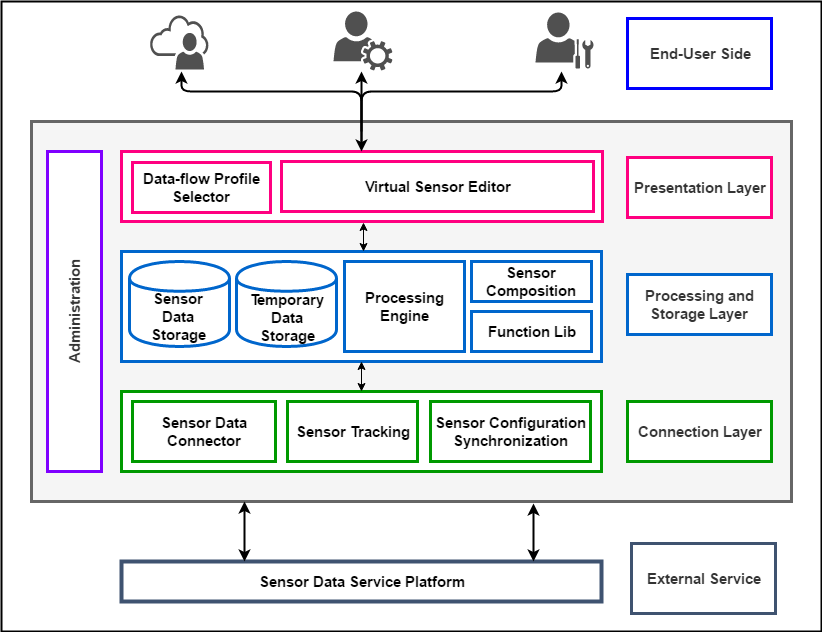
\includegraphics[width=0.72\textwidth]{./Part2/Chapter5/figures/vsf_architecture_overview.png} 
    \caption{The framework architecture overview}
     \label{fig:c5_vsf_architecture_overview}
  \end{center} 
\end{figure}

\subsubsection{Virtual Sensor Framework Workflow}
The overall blueprint of our sVSF workflow is shown in Fig.~\ref{fig:c5_vsf_operation_diagram} Physical sensors register their resource descriptions under CoRE Link Format~\cite{Shelby2012} with our backend. Once registered successfully, such sensors and resources are discovered through simple search queries. For instance, a query to search all the temperature sensor can be GET /rd-lookup/ep?rt=temperature. All sensing data from registered sensors will be forwarded to sVSF via SDSP. \\

In sVSF, VS function supports three types of the operator: rule, formula, and function. At the first state, the incoming data is received by connection layer. After that, this data is conveyed to Sensor Composition which handles and processes the VS operators and relationships in the logical data flow. This component also takes responsibility to convert VS operators to the proper mathematical operations and ensures it is executed in correct order in the processing engine. The conversions of VS operator into mathematical operation goes through two phases: First, the logical data flow content and sensor information are loaded into CP. More detail, as shown in Fig.~\ref{fig:c5_vsf_example}, a logical data flow comprises four VS operators, and sensor metadata are inserted in CP. Second, the particular variables of the operator are extracted and calculated by calling the corresponding functions in Function Lib Component (FL). These variables are reserved to simplify particular operations. For example, as shown in Fig.~\ref{fig:c5_vsf_example},  \$device.tank\_level\_change.data[24] represents all sensing data of “tank\_level\_change” sensor within 24 hours. After calculating, the values of special variables are added into virtual sensor operator before storing in temporary data storage in order to be reused in another stage. The lifetime of this temporary data can be set up by the sVSF administrators In the case of the virtual sensor has an input from another virtual sensor. This input value is also considered as a special variable and directly access via sensor name. For instance, sensor named “tank\_volume” can use the output value of “tank\_level” sensor via declaring a speacial variable named “tank\_level”. Furthermore, to maximize performance, Sensor Composition take responsibility for organizing the working schedule based on the asynchronous model. The un-relational virtual sensors, which are not linked together, will be arranged into the same thread and executed in parallel in processing engine. For example, in Fig.~\ref{fig:c5_vsf_editor_interface}, all green virtual sensors will be performed in parallel. \\

\begin{figure}[h!] 
 \begin{center} 
 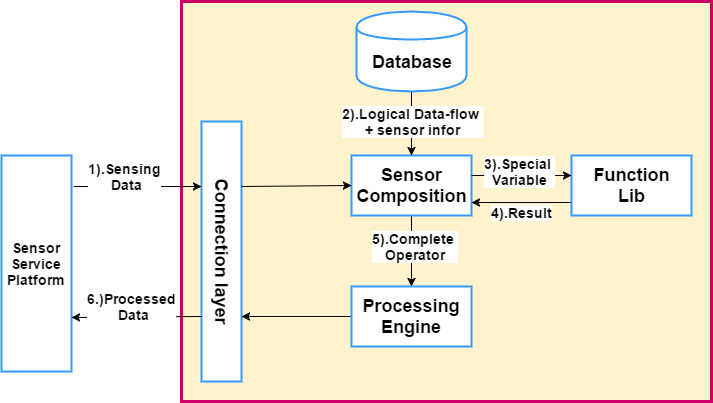
\includegraphics[width=0.72\textwidth]{./Part2/Chapter5/figures/vsf_operation_diagram.png} 
    \caption{The framework operation diagram}
     \label{fig:c5_vsf_operation_diagram}
  \end{center} 
\end{figure}

The most important component in processing layer is processing engine, where VS operators are executed. These executions are performed in parallel by a JavaScript library, namely MathJS . Finally, the output of processing engine will be stored in the database to be reused before responding final result to SDSP.


\subsection{Virtual Sensor Editor}
One of a key element of sVSF is an HTML5 web-based virtual sensor editor, which enables cross-platform development environment. The editor is a WYSIWYG (what you see is what you get) system. This allows the user to simply build a LDF by creating, configuring and connecting VSs together. VSE is implemented using native HTML5 and JointJS  library to maximize portability and availability across various end-user platforms. There are four highlighted attributes of this editor: (i) drag-drop interface: The end-user is able to simply create and link the virtual sensors by drag-drop action. (ii) Real-time Evaluation: After creating, user-defined LDF could be evaluated and receive result immediately. (iii) Reusability: VS configuration and LDF is stored and shared between the end-users. \\

\begin{figure}[h!] 
 \begin{center} 
 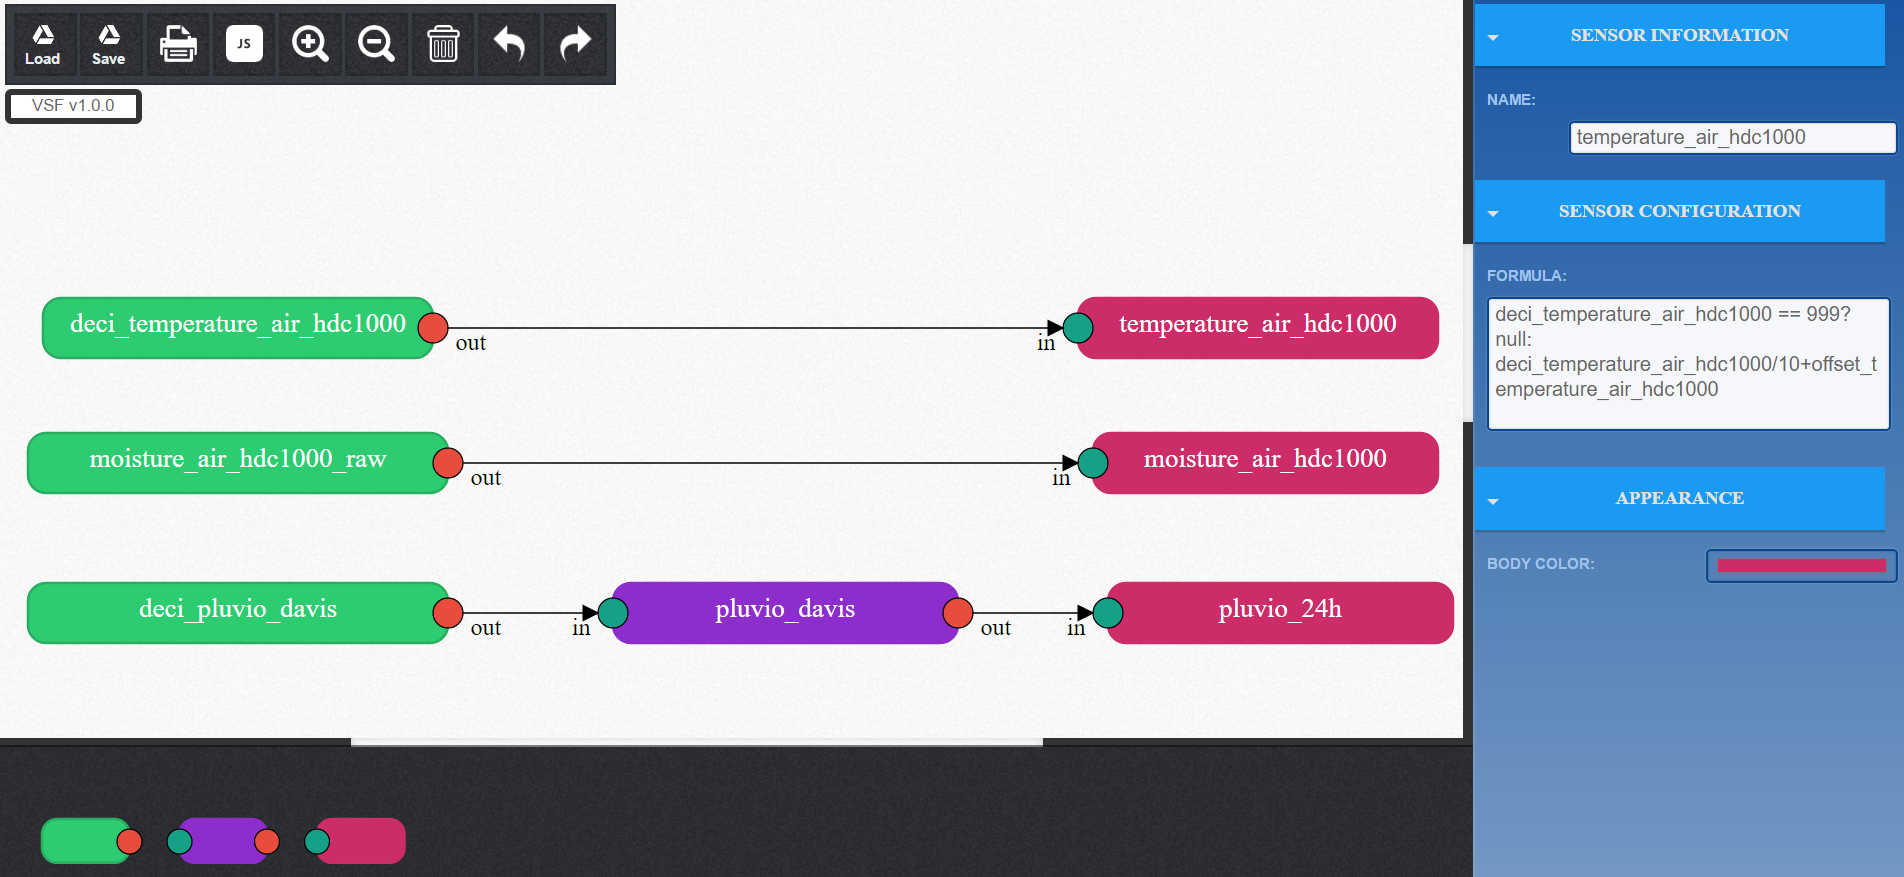
\includegraphics[width=\textwidth]{./Part2/Chapter5/figures/vsf_editor_interface.png} 
    \caption{Virtual Sensor Editor Interface}
     \label{fig:c5_vsf_editor_interface}
  \end{center} 
\end{figure}

As shown in Fig.~\ref{fig:c5_vsf_editor_interface}, a virtual sensor is represented as a box consisting of input, output ports and a VS operator. The number of these ports and sensor configuration depend on the type of virtual sensor. For example, a singular virtual sensor which serves as a physical sensor has one output and no input port. In Configuration panel on the left side, a drop box is added to allow the user to configure sensor driver. By default, we use the green and red color to identify virtual sensor type. But the end-user can change this attribute. Each output port can be assigned to one or more input of different boxes via data links. After data link is established, the later sensor enables to select the output of former sensor as an input parameter for its operator. The auto-complete feature is also equipped to speed up this selecting process. \\

Our sVSF offers recursive composing for the virtual sensor. A defined virtual sensor can be used as an input to construct other virtual sensors. After logical data flow is completely established, the evaluation feature enables the user to execute the data flow on self-generated data and receive the result immediately. Thus, the user can evaluate or correct the configuration in case of error. At the final state, the complete logical data flow is saved in the database and reused for next time.


\section{Evaluate}
In this section, we describe the utilization of our framework in a practical use-case. We also discuss how to archive high performance, scalability in our framework. Finally, an evaluation of our strategies is proposed.\\

\begin{figure}[h!] 
 \begin{center} 
 \includegraphics[width=0.95\textwidth]{./Part2/Chapter5/figures/vsf_example.png} 
    \caption{The generating high-level information process.}
     \label{fig:c5_vsf_example}
  \end{center} 
\end{figure}

Our first work has been applied to an industrial project for tank monitoring. The primary goal of this project is to manage the chemical volume via a level sensor which is plugged at the top of a tank.  The raw data of this sensor is the distance from the top of the tank to the chemical surface. Fig.~\ref{fig:c5_vsf_editor_interface} illustrates the whole process of generating high-level information such as remaining of the chemical level (Tank\_level), remains of chemical volume (Tank\_volume), change of chemical level (Tank\_level\_change), average on this change within 24h (Avg\_tank\_level\_change). Firstly, the raw data contains sensor information and sensed data is sent to sVSF. This data is handled by Sensor Composition where corresponding logical data-flow and sensor metadata is loaded from the database. In this case, the metadata is the tank information such as the height of tank (Tank\_high) and the total volume of tank (Tank\_total\_volume). At this component, special variables such as last value of such sensor (Tank\_leve.lastValue) or historical sensing data within 24h (Tank\_leve\_change.data[24]) are calculated by calling the corresponding functions in Function Lib component. All obtained information (special variable value, raw data value, sensor metadata) is injected into logical data low. Before transferring and executing at Processing Engine, logical data flow is converted to the mathematical operations. The final result is responded to SDSP via Connection Layer\\

SVSF is developed by integrating MathJS library into NodeJS Express framework  which uses event-driven architecture. Nodejs also leverages a non-blocking I/O model that allows request being processed asynchronously. In order to enhance the framework scalability, we use clustering architecture. A cluster comprises a set of servers running simultaneously. Each server is called node. The cluster is elastic to adapt to the unexpected change in term of the number of concurrent user by dynamically add or remove a node to the cluster. There are two types of nodes: master node and worker node. The master node is used to manage the worker node in the cluster. It plays a role to distribute requests among different nodes in the cluster. Other strategies are proposed to increase the performance:
\begin{itemize}
    \item The first strategy is to store the output of the virtual sensor in a temporary database. Such value could be re-used as the input of other VS sensor instead of re-calculation.
    \item The second strategy is to use an in-memory database  to speed up data querying process. Our framework uses a NoSQL database named Apache CouchDB . Comparing with a relational database, CouchDB stores the data in an independent document and its self-contained schema. As the result, it provides a massive scalability and powerful full-text search
    \item The final strategy is to apply the asynchronous model to execute logical data-flow, meaning that all independent virtual sensor or virtual sensor in the same stage is executed in parallel.
\end{itemize}
To evaluate the effectiveness of proposed strategies, we have to consider two scenarios: (i) Significantly increasing the number of simultaneous physical sensor in SDSP. (ii) Increasing the complexity of logical data flow regarding the number of VS. All evaluations are performed on a computer with following configuration: Intel(R) Core(TM) i5-6200U CPU @ 2.30GHz, 2401 MHz, 2 Core(s), 4 Logical Processor(s), 8GB of RAM and the operating system is 64-bit Windows 10. The clustering model is set up and deployed using native Clustering Module  provided by NodeJS .The data rate of the physical sensor is one message per second. For the first scenario, we have conducted an experiment with different scale of sensor network, which increases from 100 to 450 concurrent physical sensors. The logical data flow comprises 50 virtual sensors. Fig.~\ref{fig:c5_vsf_performance} illustrates the performance changes after adopting our enhancements. As shown in the figure, our enhancement is remarkably effective. Without clustering model and enhancement strategies, the response time is significant increase when expanding the scale of sensor network. After applying clustering model using 4 or 8 clusters, the response time is highly stable under 1 second regardless the size of sensor network. With 450 concurrent physical sensors, the normal response time is over 6 seconds comparing with 875 milliseconds and 650 milliseconds of the model using 4 and 8 clusters respectively.\\

\begin{figure}[h!] 
 \begin{center} 
 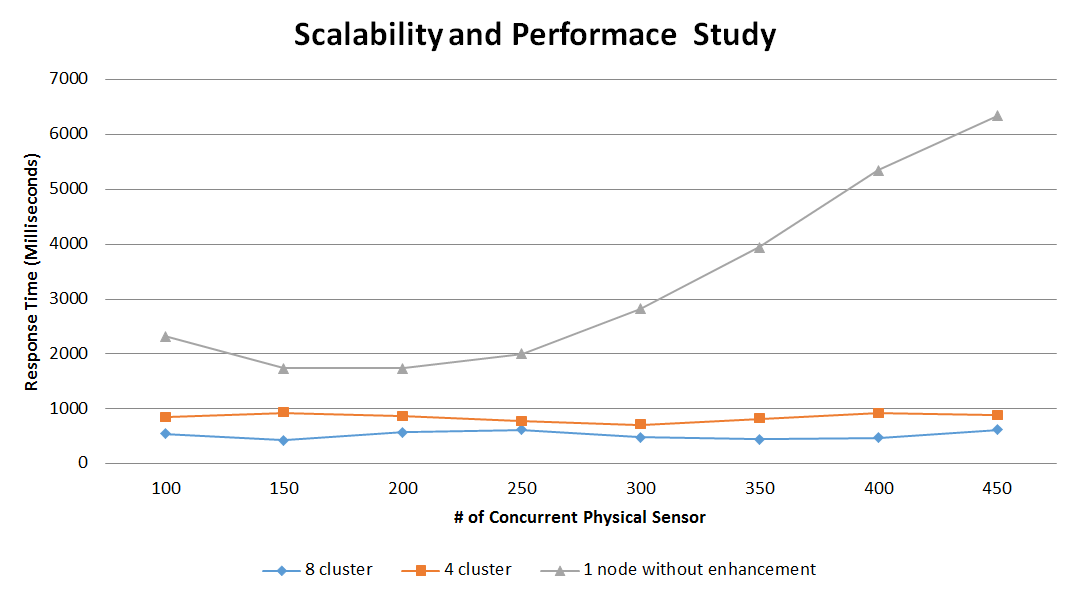
\includegraphics[width=0.9\textwidth]{./Part2/Chapter5/figures/vsf_scalability.png} 
    \caption{The effect of our enhancement in scalability and performance}
     \label{fig:c5_vsf_scalability}
  \end{center} 
\end{figure}

In the second scenario, the simulations are performed with different logical data flows size, which contains from 1 to 100 virtual sensors. Each logical data-flow is evaluated by various sensor network scale in SDSP. As shown in Fig.~\ref{fig:c5_vsf_scalability}, when increasing the number of concurrent physical sensor, the response time lightly increases regardless logical data flow size. In case the scale of the logical data flow is moderate (comprising under 50 virtual sensors), our system is able to serve a data message under 800ms even when 50 concurrent physical sensors are running. In the case of scaling up to 100 concurrent physical sensors, the response time is still under  1 second.

\begin{figure}[h!] 
 \begin{center} 
 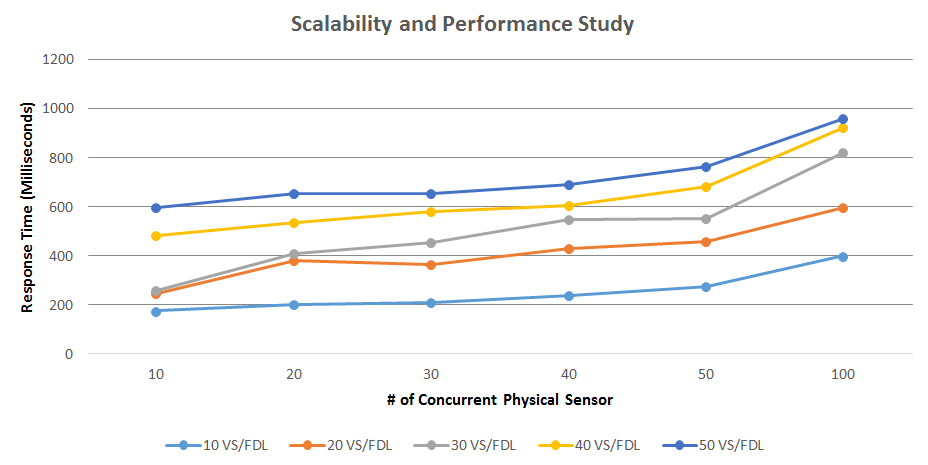
\includegraphics[width=0.9\textwidth]{./Part2/Chapter5/figures/vsf_performance.png} 
    \caption{The framework’s performance}
     \label{fig:c5_vsf_performance}
  \end{center} 
\end{figure}

\section{Results and discussion}
In this paper, we review a concept of the virtual sensor and propose a new virtual sensor taxonomy based on its functionality. The limitations of the existing virtual sensor frameworks are also considered in term of virtual sensor functionality and usability. Motivating to bridge the gaps, we proposed a scalable virtual sensor framework that allows producing high-level information from sensed data, by creating a logical data flow over a collection of the virtual sensor. A web-based virtual sensor editor is also offered to accelerate creating and configuring logical data-flow. In evaluation section, a serial of strategies to enhance the performance and scalability are discussed and evaluated. Regarding future works, we are currently working on integrating our platform into the oneM2M based framework~\cite{DattaGyrardBonnetBoudaoud2015} and FIWARE  architecture for ensuring interoperability.
\section{Conclusion}
